\documentclass{standalone}
\usepackage{tikz}
\usetikzlibrary{decorations.markings}
\usetikzlibrary{positioning}

\definecolor{gray}{RGB}{126, 126, 126}
\definecolor{orange}{RGB}{252, 234, 220}
\definecolor{flieder}{RGB}{237, 233, 241}
\definecolor{lightgreen}{RGB}{234, 240, 222}
\definecolor{pink}{RGB}{241, 219, 217}
\definecolor{lightblue}{RGB}{233, 238, 244}

\newlength{\nodedist}   
\setlength{\nodedist}{0.4cm}  
\newlength{\halfnodedist}   
\setlength{\halfnodedist}{0.2cm}  
\def\looseness{3}

\newsavebox{\mybox}
\begin{document}
\sbox{\mybox}{
\begin{tikzpicture}

\node[rectangle, draw=gray, fill=orange](a)[]{3 conv, 32, /2};
\node[rectangle, draw=gray, fill=orange](b)[below=\nodedist of a]{3 conv, 32};
\node[rectangle, draw=gray, fill=orange](c)[below=\nodedist of b]{3 conv, 64};
\node[rectangle](pool)[below=\nodedist of c]{pool, /2};
\draw[->] (a.south) -- (b.north);
\draw[->] (b.south) -- (c.north);
\draw[-] (c.south) -- (pool.north);


\node[](skip1)[below=\halfnodedist of pool]{};
\draw[-] (pool.south) -- (skip1.center);
\node[rectangle, draw=gray, fill=flieder](a)[below=\halfnodedist of skip1]{3 conv, 64};
\node[rectangle, draw=gray, fill=flieder](b)[below=\nodedist of a]{3 conv, 64};
\node[](skip2)[below=\halfnodedist of b]{};
\draw[->] (skip1.center) -- (a.north);
\draw[->] (a.south) -- (b.north);
\draw[-] (b.south) -- (skip2.center);
\begin{scope}[decoration={markings,mark=at position 0.5 with {\arrow{>}}}] 
    \draw[postaction={decorate}] (skip1.center) to[out=0, in=0, looseness=\looseness] (skip2.center);
\end{scope}
\node[](skip1) at (skip2) {};

\node[rectangle, draw=gray, fill=flieder](a)[below=\halfnodedist of skip1]{3 conv, 64};
\node[rectangle, draw=gray, fill=flieder](b)[below=\nodedist of a]{3 conv, 64};
\node[](skip2)[below=\halfnodedist of b]{};
\draw[->] (skip1.center) -- (a.north);
\draw[->] (a.south) -- (b.north);
\draw[-] (b.south) -- (skip2.center);
\begin{scope}[decoration={markings,mark=at position 0.5 with {\arrow{>}}}] 
    \draw[postaction={decorate}] (skip1.center) to[out=0, in=0, looseness=\looseness] (skip2.center);
\end{scope}
\node[](skip1) at (skip2) {};

\node[rectangle, draw=gray, fill=flieder](a)[below=\halfnodedist of skip1]{3 conv, 64};
\node[rectangle, draw=gray, fill=flieder](b)[below=\nodedist of a]{3 conv, 64};
\node[](skip2)[below=\halfnodedist of b]{};
\draw[->] (skip1.center) -- (a.north);
\draw[->] (a.south) -- (b.north);
\draw[-] (b.south) -- (skip2.center);
\begin{scope}[decoration={markings,mark=at position 0.5 with {\arrow{>}}}] 
    \draw[postaction={decorate}] (skip1.center) to[out=0, in=0, looseness=\looseness] (skip2.center);
\end{scope}
\node[](skip1) at (skip2) {};


\node[rectangle, draw=gray, fill=lightgreen](a)[below=\halfnodedist of skip1]{3 conv, 128, /2};
\node[rectangle, draw=gray, fill=lightgreen](b)[below=\nodedist of a]{3 conv, 128};
\node[](skip2)[below=\halfnodedist of b]{};
\draw[->] (skip1.center) -- (a.north);
\draw[->] (a.south) -- (b.north);
\draw[-] (b.south) -- (skip2.center);
\begin{scope}[decoration={markings,mark=at position 0.5 with {\arrow{>}}}] 
    \draw[dashed,postaction={decorate}] (skip1.center) to[out=0, in=0, looseness=\looseness] (skip2.center);
\end{scope}
\node[](skip1) at (skip2) {};

\node[rectangle, draw=gray, fill=lightgreen](a)[below=\halfnodedist of skip1]{3 conv, 128};
\node[rectangle, draw=gray, fill=lightgreen](b)[below=\nodedist of a]{3 conv, 128};
\node[](skip2)[below=\halfnodedist of b]{};
\draw[->] (skip1.center) -- (a.north);
\draw[->] (a.south) -- (b.north);
\draw[-] (b.south) -- (skip2.center);
\begin{scope}[decoration={markings,mark=at position 0.5 with {\arrow{>}}}] 
    \draw[postaction={decorate}] (skip1.center) to[out=0, in=0, looseness=\looseness] (skip2.center);
\end{scope}
\node[](skip1) at (skip2) {};

\node[rectangle, draw=gray, fill=lightgreen](a)[below=\halfnodedist of skip1]{3 conv, 128};
\node[rectangle, draw=gray, fill=lightgreen](b)[below=\nodedist of a]{3 conv, 128};
\node[](skip2)[below=\halfnodedist of b]{};
\draw[->] (skip1.center) -- (a.north);
\draw[->] (a.south) -- (b.north);
\draw[-] (b.south) -- (skip2.center);
\begin{scope}[decoration={markings,mark=at position 0.5 with {\arrow{>}}}] 
    \draw[postaction={decorate}] (skip1.center) to[out=0, in=0, looseness=\looseness] (skip2.center);
\end{scope}
\node[](skip1) at (skip2) {};

\node[rectangle, draw=gray, fill=lightgreen](a)[below=\halfnodedist of skip1]{3 conv, 128};
\node[rectangle, draw=gray, fill=lightgreen](b)[below=\nodedist of a]{3 conv, 128};
\node[](skip2)[below=\halfnodedist of b]{};
\draw[->] (skip1.center) -- (a.north);
\draw[->] (a.south) -- (b.north);
\draw[-] (b.south) -- (skip2.center);
\begin{scope}[decoration={markings,mark=at position 0.5 with {\arrow{>}}}] 
    \draw[postaction={decorate}] (skip1.center) to[out=0, in=0, looseness=\looseness] (skip2.center);
\end{scope}
\node[](skip1) at (skip2) {};


\node[rectangle, draw=gray, fill=pink](a)[below=\halfnodedist of skip1]{3 conv, 256, /2};
\node[rectangle, draw=gray, fill=pink](b)[below=\nodedist of a]{3 conv, 256};
\node[](skip2)[below=\halfnodedist of b]{};
\draw[->] (skip1.center) -- (a.north);
\draw[->] (a.south) -- (b.north);
\draw[-] (b.south) -- (skip2.center);
\begin{scope}[decoration={markings,mark=at position 0.5 with {\arrow{>}}}] 
    \draw[dashed,postaction={decorate}] (skip1.center) to[out=0, in=0, looseness=\looseness] (skip2.center);
\end{scope}
\node[](skip1) at (skip2) {};

\node[rectangle, draw=gray, fill=pink](a)[below=\halfnodedist of skip1]{3 conv, 256};
\node[rectangle, draw=gray, fill=pink](b)[below=\nodedist of a]{3 conv, 256};
\node[](skip2)[below=\halfnodedist of b]{};
\draw[->] (skip1.center) -- (a.north);
\draw[->] (a.south) -- (b.north);
\draw[-] (b.south) -- (skip2.center);
\begin{scope}[decoration={markings,mark=at position 0.5 with {\arrow{>}}}] 
    \draw[postaction={decorate}] (skip1.center) to[out=0, in=0, looseness=\looseness] (skip2.center);
\end{scope}
\node[](skip1) at (skip2) {};

\node[rectangle, draw=gray, fill=pink](a)[below=\halfnodedist of skip1]{3 conv, 256};
\node[rectangle, draw=gray, fill=pink](b)[below=\nodedist of a]{3 conv, 256};
\node[](skip2)[below=\halfnodedist of b]{};
\draw[->] (skip1.center) -- (a.north);
\draw[->] (a.south) -- (b.north);
\draw[-] (b.south) -- (skip2.center);
\begin{scope}[decoration={markings,mark=at position 0.5 with {\arrow{>}}}] 
    \draw[postaction={decorate}] (skip1.center) to[out=0, in=0, looseness=\looseness] (skip2.center);
\end{scope}
\node[](skip1) at (skip2) {};

\node[rectangle, draw=gray, fill=pink](a)[below=\halfnodedist of skip1]{3 conv, 256};
\node[rectangle, draw=gray, fill=pink](b)[below=\nodedist of a]{3 conv, 256};
\node[](skip2)[below=\halfnodedist of b]{};
\draw[->] (skip1.center) -- (a.north);
\draw[->] (a.south) -- (b.north);
\draw[-] (b.south) -- (skip2.center);
\begin{scope}[decoration={markings,mark=at position 0.5 with {\arrow{>}}}] 
    \draw[postaction={decorate}] (skip1.center) to[out=0, in=0, looseness=\looseness] (skip2.center);
\end{scope}
\node[](skip1) at (skip2) {};

\node[rectangle, draw=gray, fill=pink](a)[below=\halfnodedist of skip1]{3 conv, 256};
\node[rectangle, draw=gray, fill=pink](b)[below=\nodedist of a]{3 conv, 256};
\node[](skip2)[below=\halfnodedist of b]{};
\draw[->] (skip1.center) -- (a.north);
\draw[->] (a.south) -- (b.north);
\draw[-] (b.south) -- (skip2.center);
\begin{scope}[decoration={markings,mark=at position 0.5 with {\arrow{>}}}] 
    \draw[postaction={decorate}] (skip1.center) to[out=0, in=0, looseness=\looseness] (skip2.center);
\end{scope}
\node[](skip1) at (skip2) {};

\node[rectangle, draw=gray, fill=pink](a)[below=\halfnodedist of skip1]{3 conv, 256};
\node[rectangle, draw=gray, fill=pink](b)[below=\nodedist of a]{3 conv, 256};
\node[](skip2)[below=\halfnodedist of b]{};
\draw[->] (skip1.center) -- (a.north);
\draw[->] (a.south) -- (b.north);
\draw[-] (b.south) -- (skip2.center);
\begin{scope}[decoration={markings,mark=at position 0.5 with {\arrow{>}}}] 
    \draw[postaction={decorate}] (skip1.center) to[out=0, in=0, looseness=\looseness] (skip2.center);
\end{scope}
\node[](skip1) at (skip2) {};


\node[rectangle, draw=gray, fill=lightblue](a)[below=\halfnodedist of skip1]{3 conv, 512, /2};
\node[rectangle, draw=gray, fill=lightblue](b)[below=\nodedist of a]{3 conv, 64};
\node[](skip2)[below=\halfnodedist of b]{};
\draw[->] (skip1.center) -- (a.north);
\draw[->] (a.south) -- (b.north);
\draw[-] (b.south) -- (skip2.center);
\begin{scope}[decoration={markings,mark=at position 0.5 with {\arrow{>}}}] 
    \draw[dashed,postaction={decorate}] (skip1.center) to[out=0, in=0, looseness=\looseness] (skip2.center);
\end{scope}
\node[](skip1) at (skip2) {};

\node[rectangle, draw=gray, fill=lightblue](a)[below=\halfnodedist of skip2]{3 conv, 512};
\node[rectangle, draw=gray, fill=lightblue](b)[below=\nodedist of a]{3 conv, 512};
\node[](skip2)[below=\halfnodedist of b]{};
\draw[->] (skip1.center) -- (a.north);
\draw[->] (a.south) -- (b.north);
\draw[-] (b.south) -- (skip2.center);
\begin{scope}[decoration={markings,mark=at position 0.5 with {\arrow{>}}}] 
    \draw[postaction={decorate}] (skip1.center) to[out=0, in=0, looseness=\looseness] (skip2.center);
\end{scope}
\node[](skip1) at (skip2) {};

\node[rectangle, draw=gray, fill=lightblue](a)[below=\halfnodedist of skip1]{3 conv, 512};
\node[rectangle, draw=gray, fill=lightblue](b)[below=\nodedist of a]{3 conv, 512};
\node[](skip2)[below=\halfnodedist of b]{};
\draw[->] (skip1.center) -- (a.north);
\draw[->] (a.south) -- (b.north);
\draw[-] (b.south) -- (skip2.center);
\begin{scope}[decoration={markings,mark=at position 0.5 with {\arrow{>}}}] 
    \draw[postaction={decorate}] (skip1.center) to[out=0, in=0, looseness=\looseness] (skip2.center);
\end{scope}
\node[](skip1) at (skip2) {};

\node[](out)[below=\halfnodedist of skip2]{out};
\draw[->] (skip2.center) -- (out.north);

\end{tikzpicture}
}
\typeout{WIDTH=\the\wd\mybox}
\typeout{HEIGHT=\the\ht\mybox}
\usebox{\mybox}
\end{document}